\section{Dimension Reduction} \label{sec:Dimension_Reduction}

\blindtext

\begin{figure}[!hbt]
    \centering
    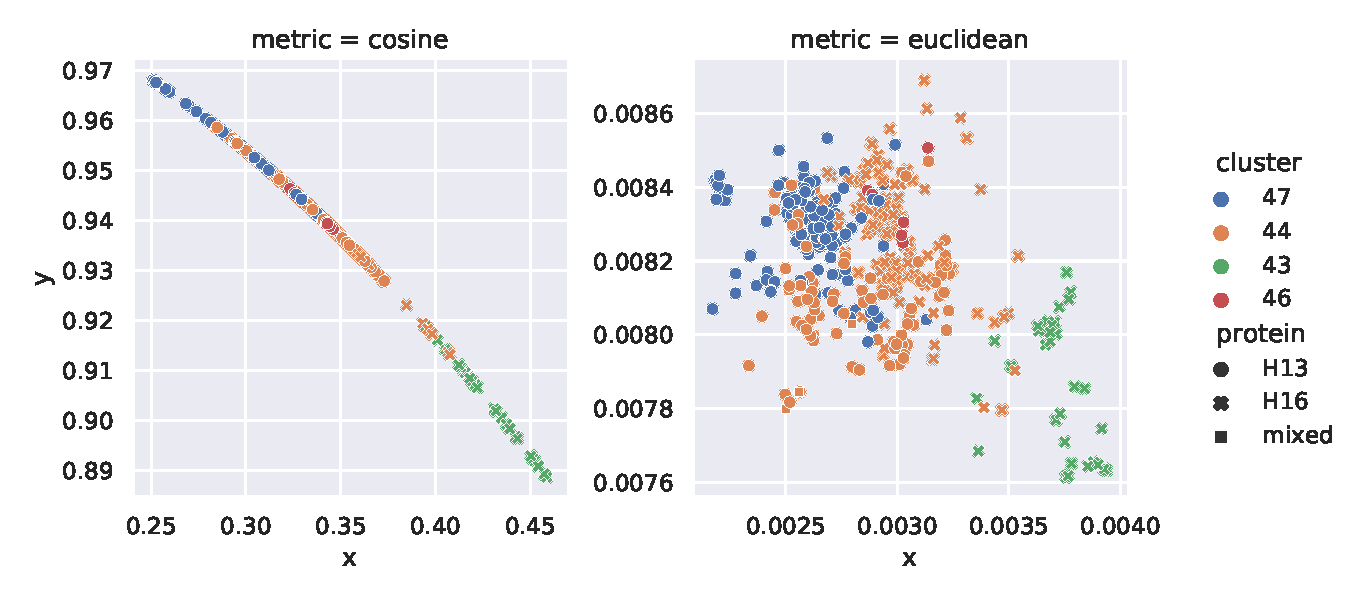
\includegraphics[width=\textwidth]{PCA/Difference_Segment_4_H_PCA.pdf}
    \caption[H13/H16 Component Reduction Example (\Acrshort{PCA})]{\textbf{H13/H16 Component Reduction Example (\Acrshort{PCA}).} .}
    \label{fig:Reduction_Example_PCA}
\end{figure}

\begin{figure}[!hbt]
    \centering
    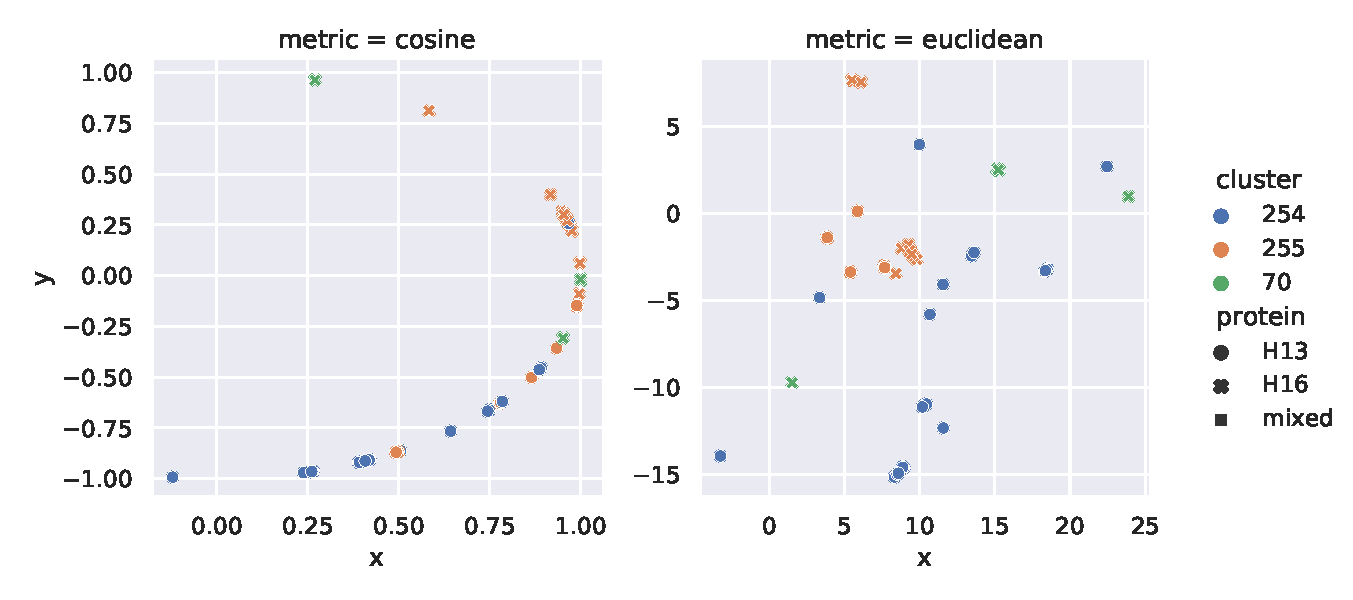
\includegraphics[width=\textwidth]{UMAP/Difference_Segment_4_H_UMAP_Neighbors_10.pdf}
    \caption[H13/H16 Component Reduction Example (\Acrshort{UMAP}, n = 10)]{\textbf{H13/H16 Component Reduction Example (\Acrshort{UMAP}, n = 10).} .}
    \label{fig:Reduction_Example_UMAP_10}
\end{figure}

\begin{figure}[!hbt]
    \centering
    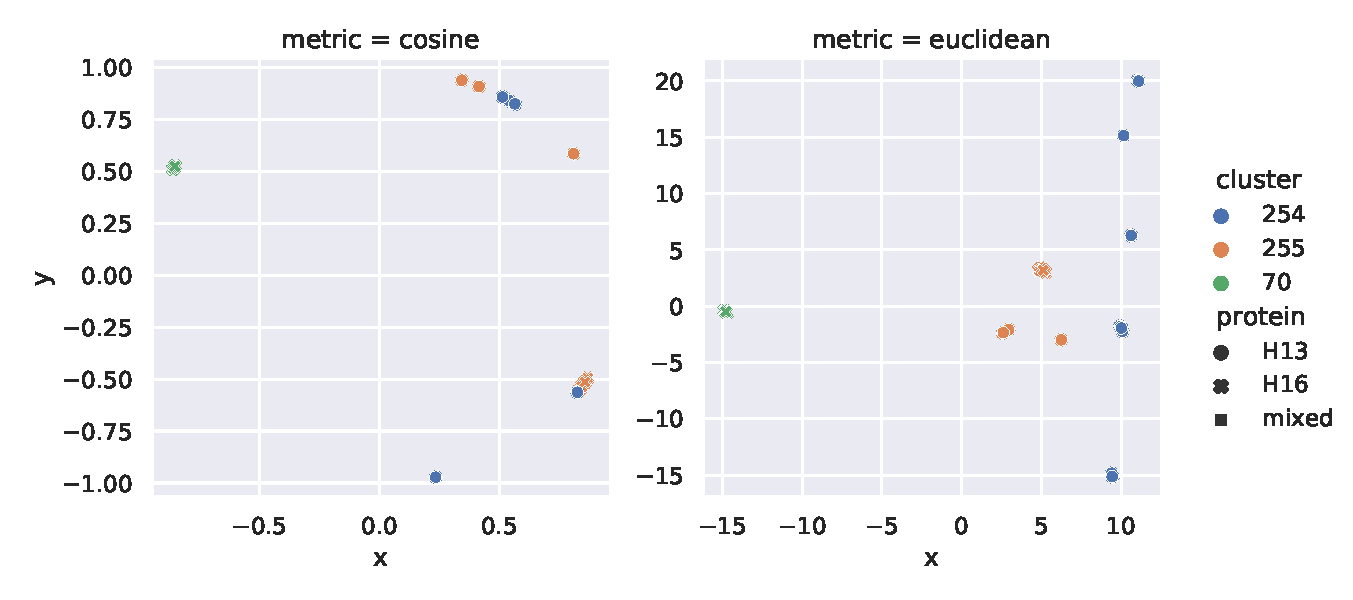
\includegraphics[width=\textwidth]{UMAP/Difference_Segment_4_H_UMAP_Neighbors_50.pdf}
    \caption[H13/H16 Component Reduction Example (\Acrshort{UMAP}, n = 50)]{\textbf{H13/H16 Component Reduction Example (\Acrshort{UMAP}, n = 50).} .}
    \label{fig:Reduction_Example_UMAP_50}
\end{figure}

\begin{figure}[!hbt]
    \centering
    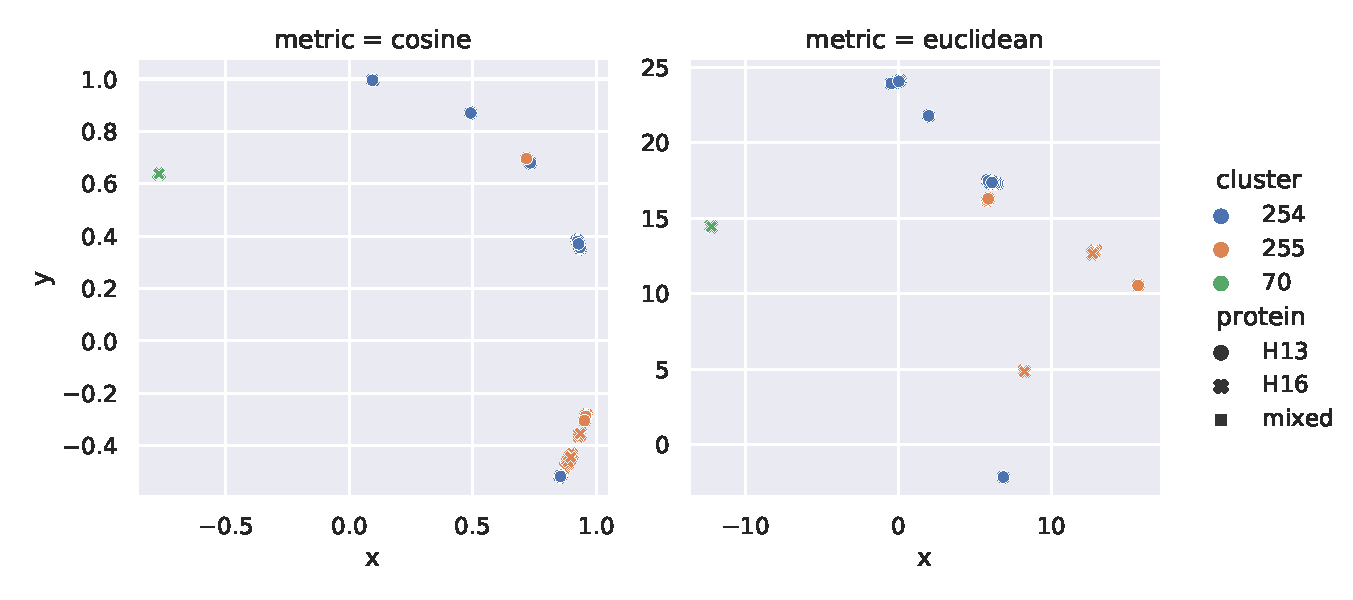
\includegraphics[width=\textwidth]{UMAP/Difference_Segment_4_H_UMAP_Neighbors_100.pdf}
    \caption[H13/H16 Component Reduction Example (\Acrshort{UMAP}, n = 100)]{\textbf{H13/H16 Component Reduction Example (\Acrshort{UMAP}, n = 100).} .}
    \label{fig:Reduction_Example_UMAP_100}
\end{figure}

\begin{figure}[!hbt]
    \centering
    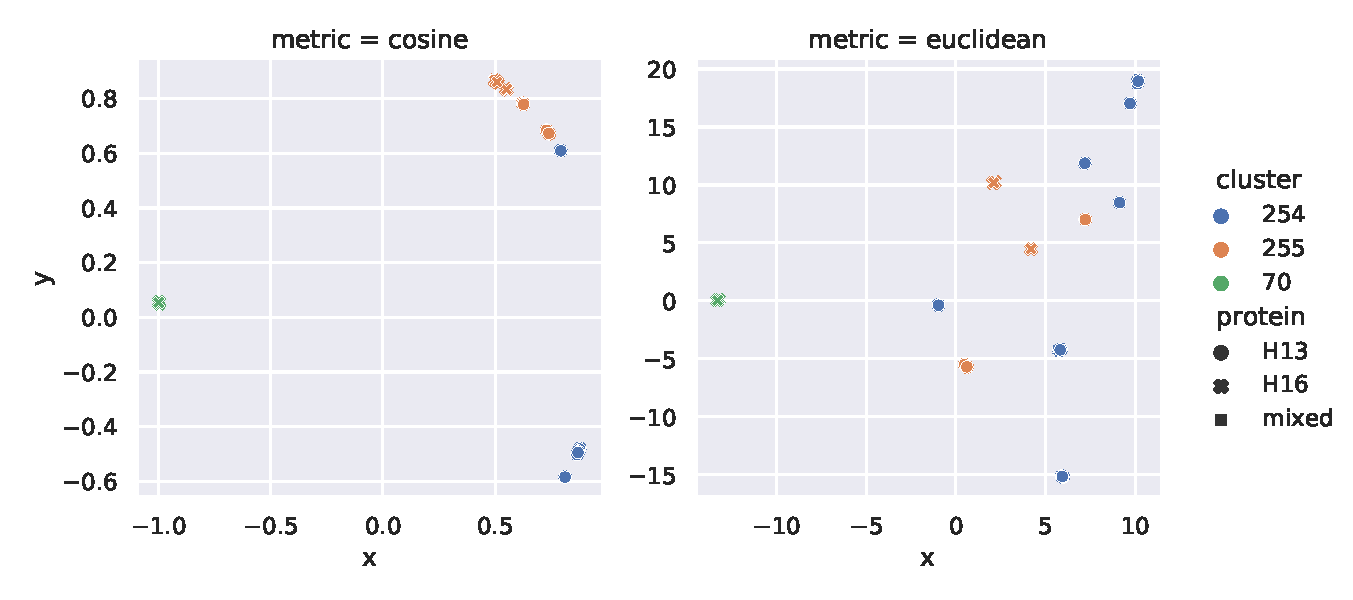
\includegraphics[width=\textwidth]{UMAP/Difference_Segment_4_H_UMAP_Neighbors_200.pdf}
    \caption[H13/H16 Component Reduction Example (\Acrshort{UMAP}, n = 200)]{\textbf{H13/H16 Component Reduction Example (\Acrshort{UMAP}, n = 200).} .}   \label{fig:Reduction_Example_UMAP_200}
\end{figure}

%wichtig erkläre warum dimension reuction mit neigbors 100 und dann feines clustering sinn macht -> HDBSCAN in methoden